% Created 2016-10-24 Mon 22:57
\documentclass[11pt]{article}
\usepackage[utf8]{inputenc}
\usepackage[T1]{fontenc}
\usepackage{fixltx2e}
\usepackage{graphicx}
\usepackage{longtable}
\usepackage{float}
\usepackage{wrapfig}
\usepackage{rotating}
\usepackage[normalem]{ulem}
\usepackage{amsmath}
\usepackage{textcomp}
\usepackage{marvosym}
\usepackage{wasysym}
\usepackage{amssymb}
\usepackage{hyperref}
\tolerance=1000
\author{Yi Ou olly93219@outlook u1010138}
\date{Jiani Lin jiani@cs.utah.edu u1011802}
\title{Insights in European league soccer players transfer \emph{\href{http://github.com/SayingsOlly/dataviscourse-pr-insights-in-European-league-soccer-transfer}{Github Link}}}
\hypersetup{
  pdfkeywords={},
  pdfsubject={},
  pdfcreator={Emacs 25.1.1 (Org mode 8.2.10)}}
\begin{document}

\maketitle
\tableofcontents


\section{Motivation}
\label{sec-1}
Enjoying watching the European soccer league games, we want to visualize data about soccer to show the trend of soccer's development.
Since there have been many research about the outcome of games, we decide to exploring our data from another perspective:
the transfer market which reflects not only the loyalty of players but also the development of leagues or teams. Our topic is the European league soccer transfer,
related to the number of players transfer both within and among leagues as well as the rank of players who has the most number of transfer times.

\section{Project Objectives}
\label{sec-2}
\begin{enumerate}
\item How many players transferd between teams within a league in each year.
\item How many players transferd between leagues in each year.
\item The trend of the number of transferd players among leagues.
\item The rank of players who has the most number of transfer times.
\end{enumerate}
\section{Data}
\label{sec-3}

Our data is from Kaggle European Soccer Database, and the link is \emph{\href{https://www.kaggle.com/hugomathien/soccer}{here}}.\\
\\
The data we want to use has 11 European league, more than 25000 matches and at least 10000 players from season 2008 to season 2016.\\
\\
The form of data set is several tables in sqlite database, so we plan to join the tables to get which player belongs to which team from year to year, then we can know the trasfer of players.\\


\section{Design}
\label{sec-4}



\subsection{Brain Storm}
\label{sec-4-1}

\begin{itemize}
\item Brain Storm1:
\end{itemize}
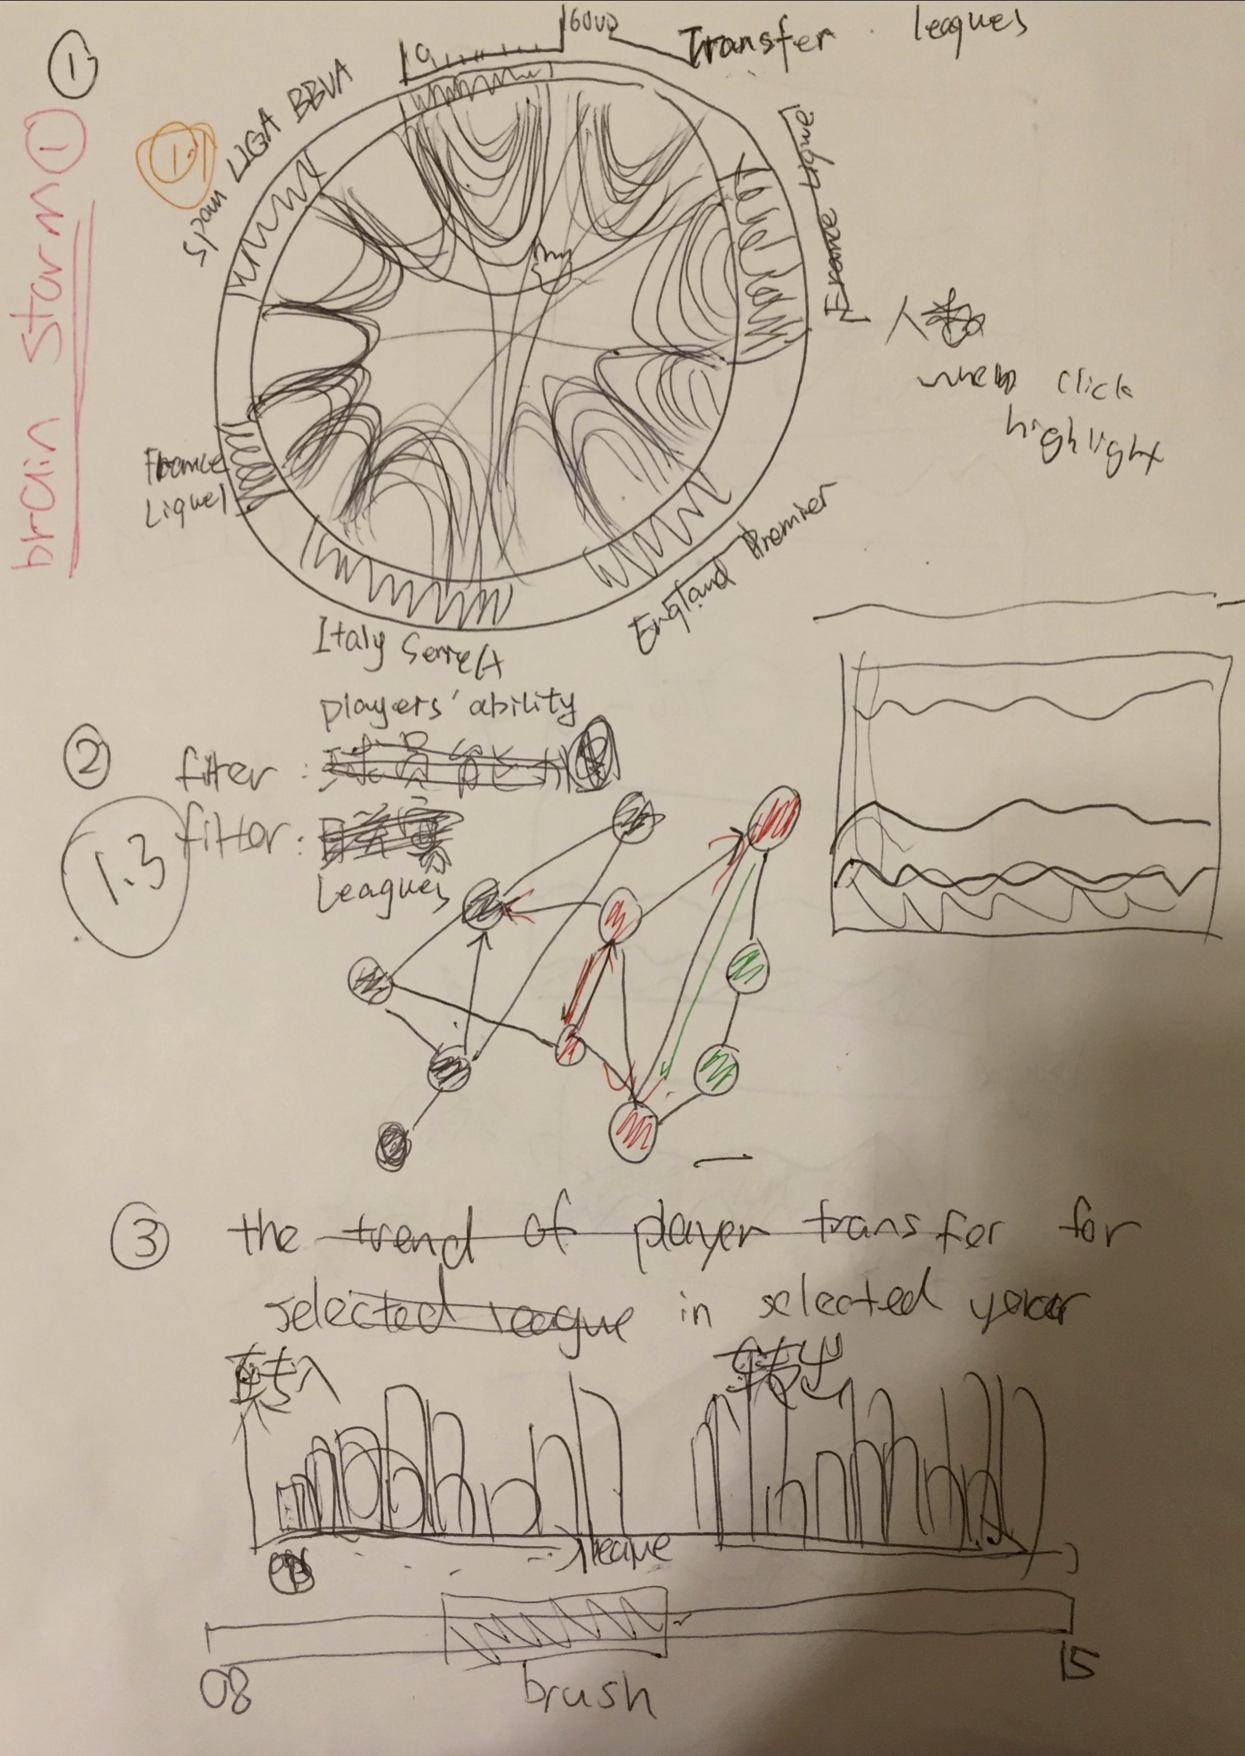
\includegraphics[width=.9\linewidth]{Design.png}

\begin{itemize}
\item Brain Storm2:
\end{itemize}
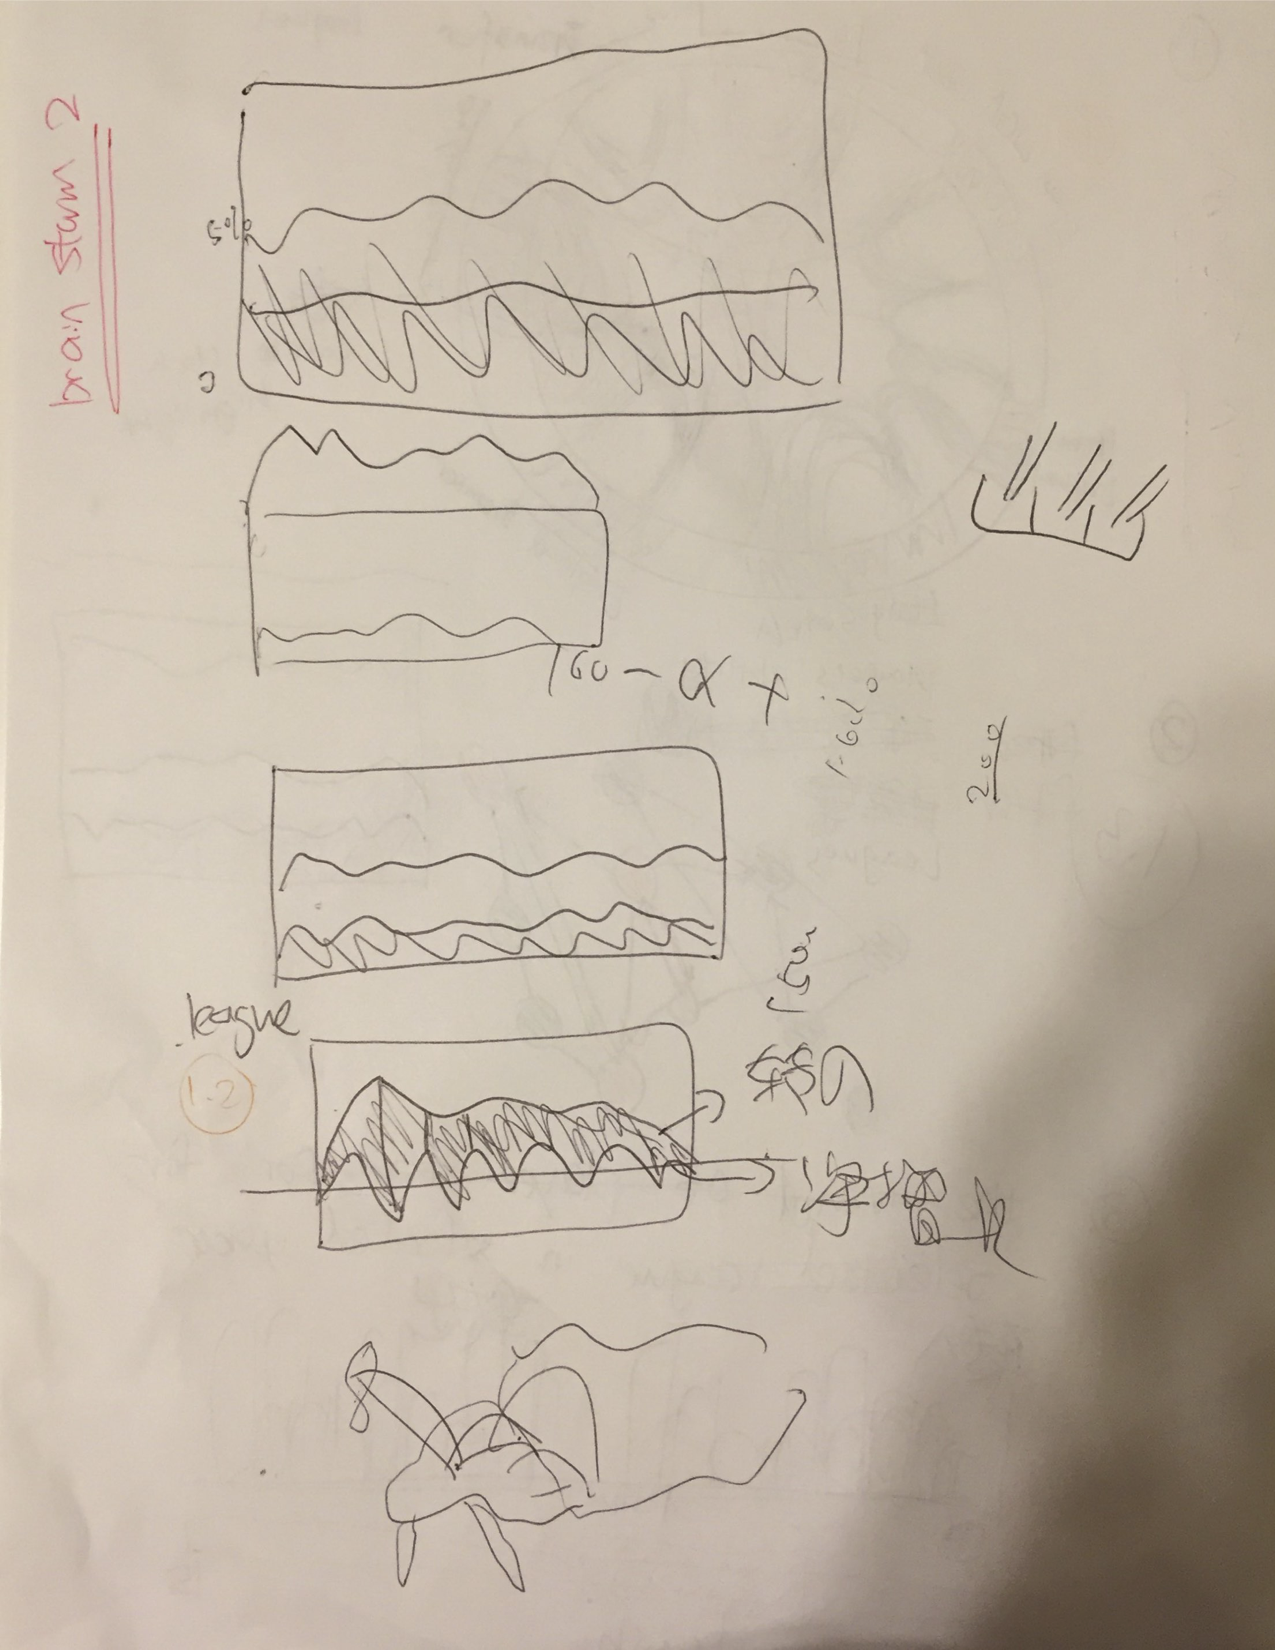
\includegraphics[width=.9\linewidth]{Design2.png}

\begin{itemize}
\item Brian Storm3:
\end{itemize}
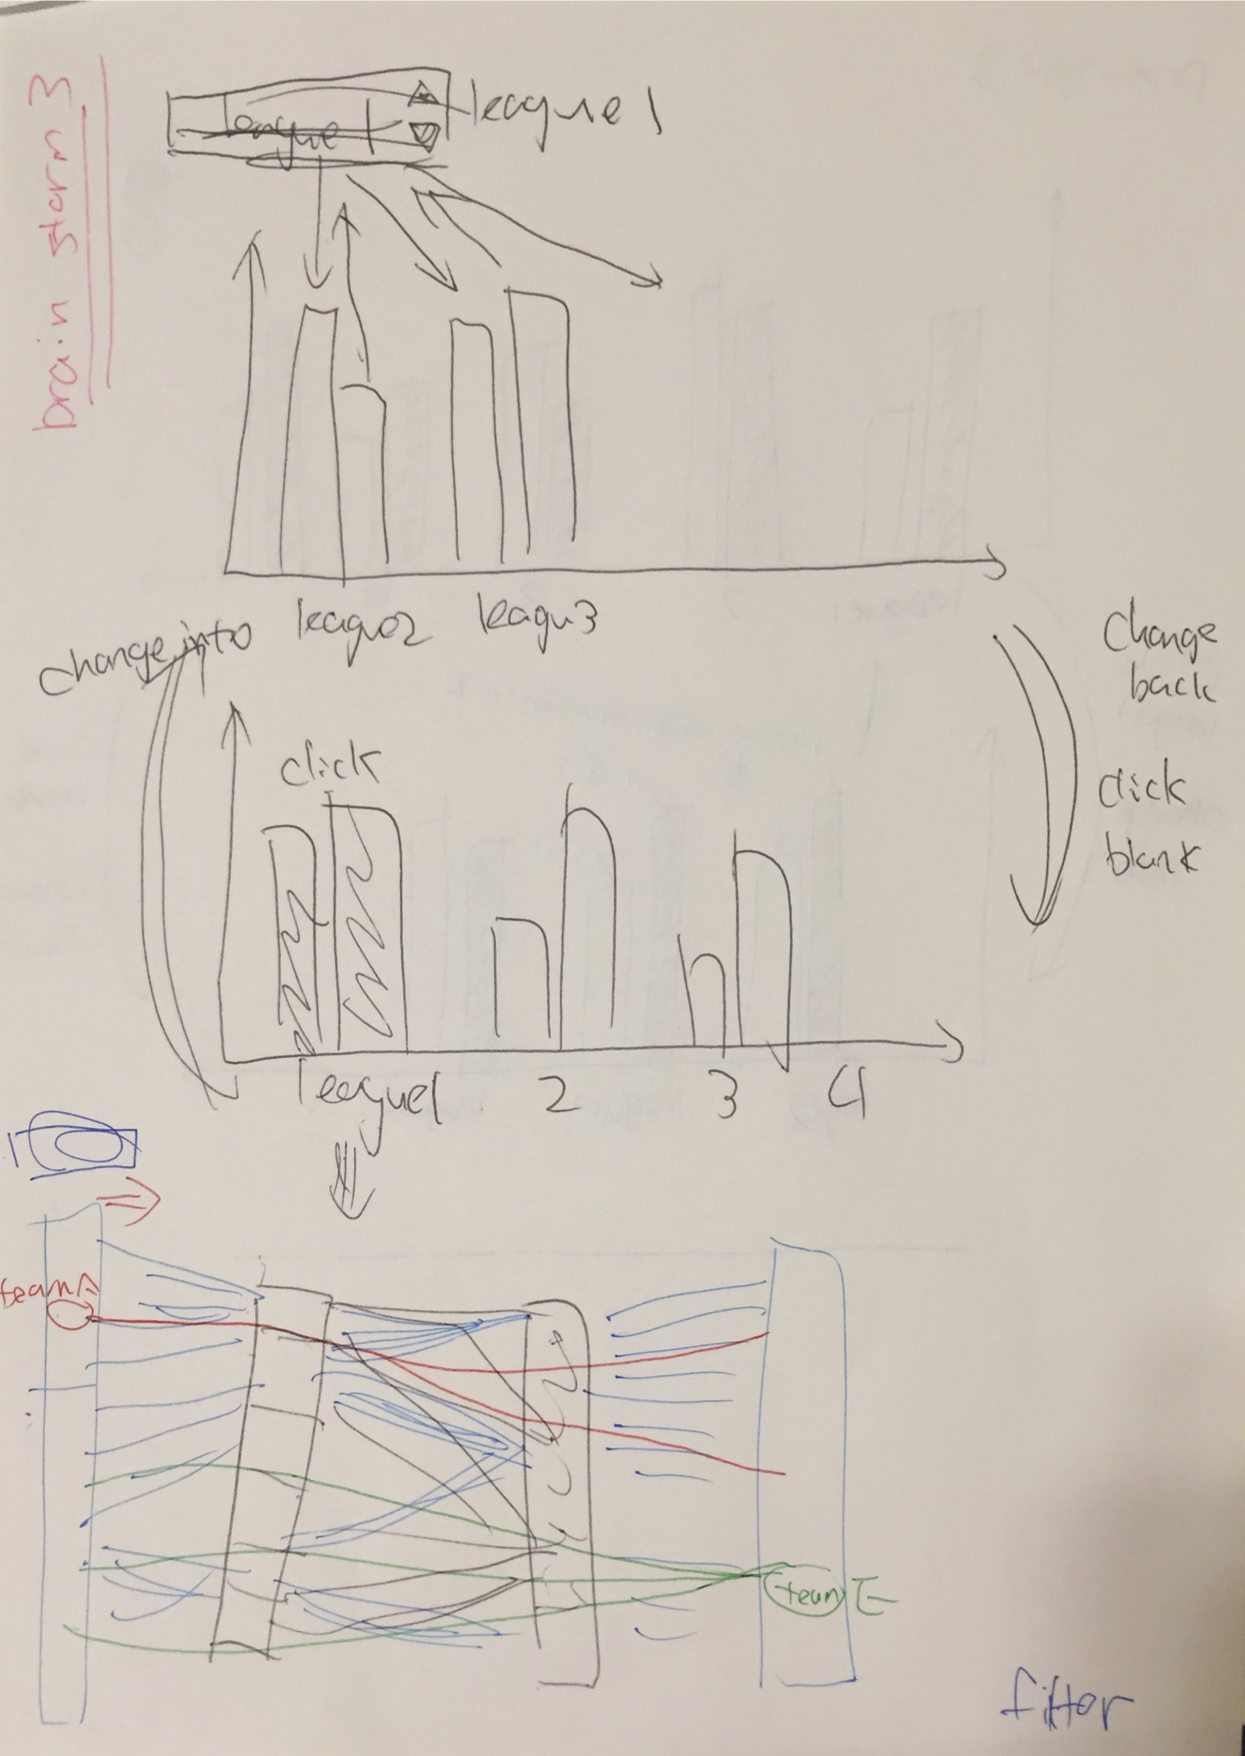
\includegraphics[width=.9\linewidth]{Design3.png}
\subsection{Initial Design}
\label{sec-4-2}

\begin{itemize}
\item Design1:
\end{itemize}
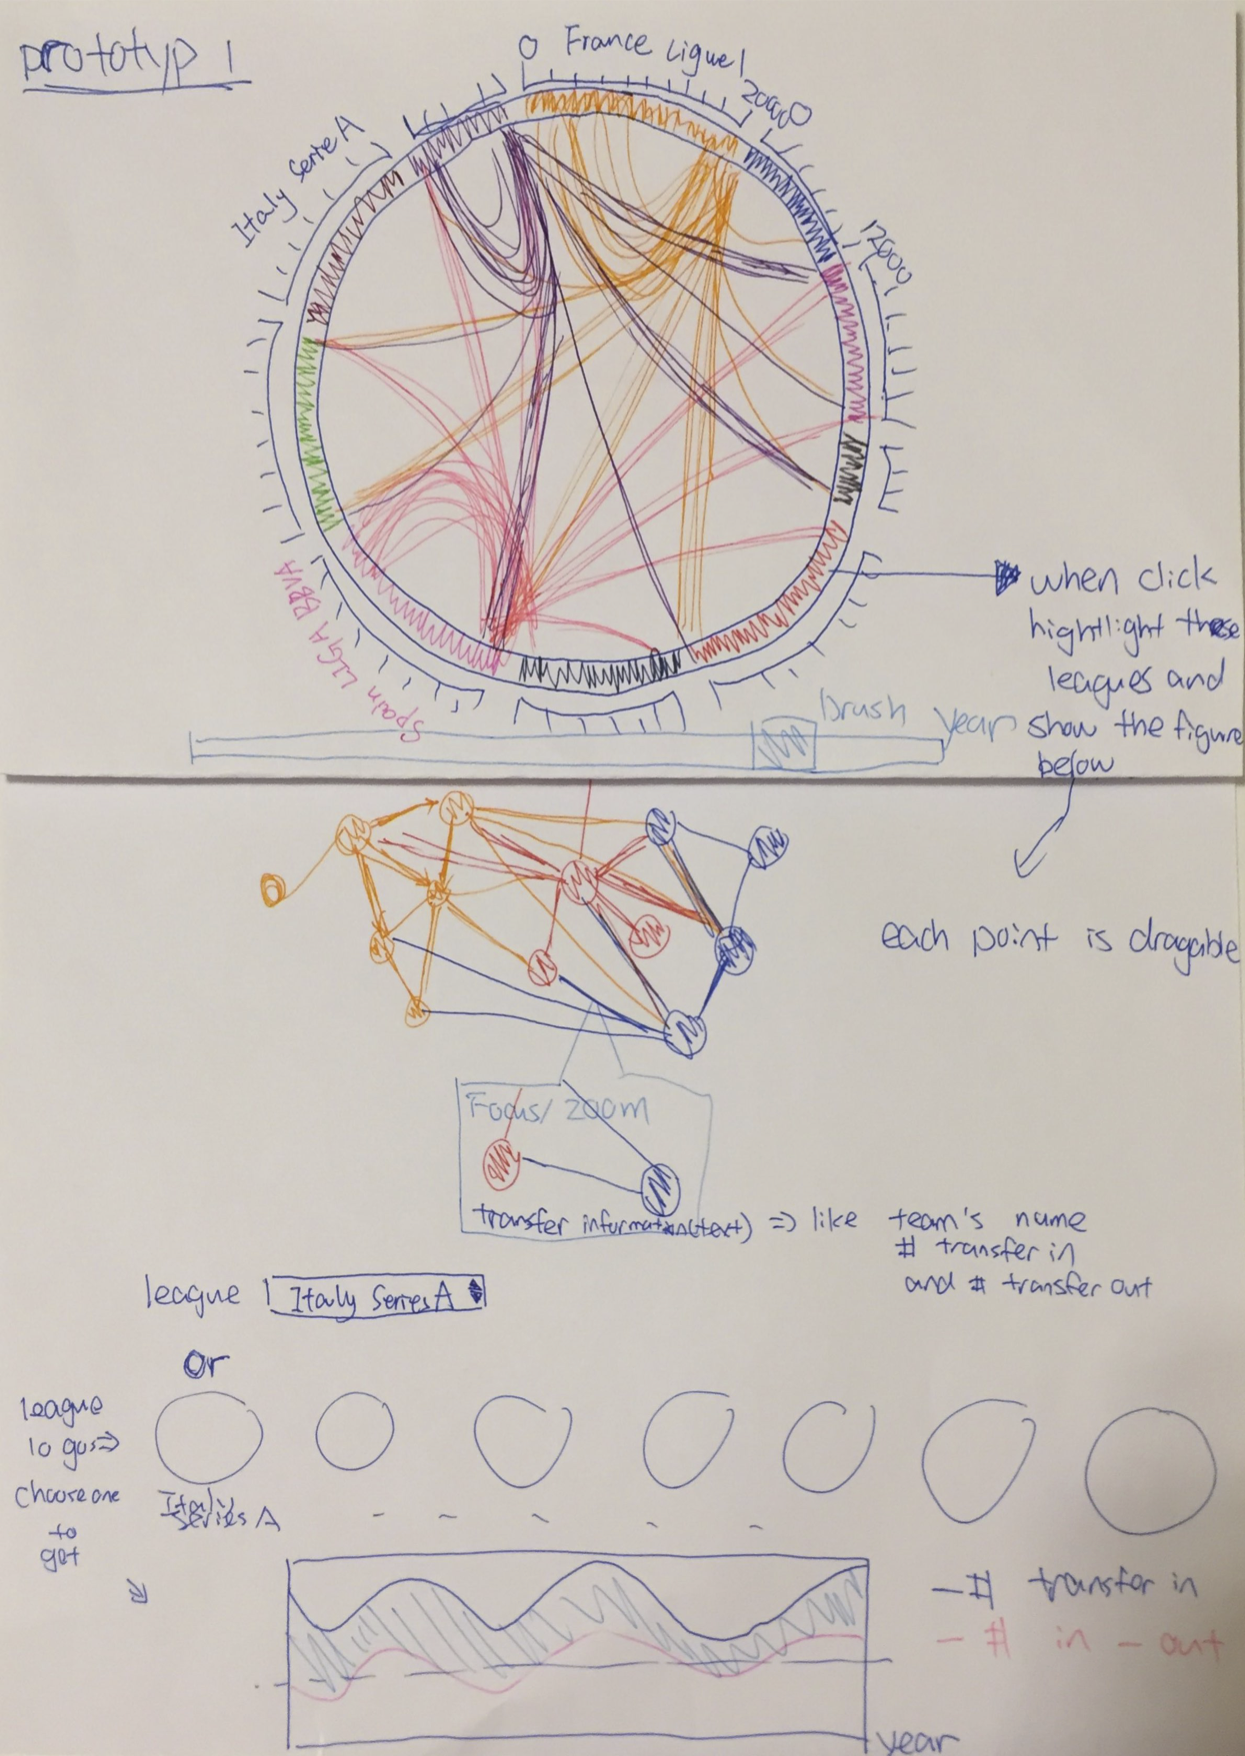
\includegraphics[width=.9\linewidth]{Design4.png}

\begin{itemize}
\item Design2:
\end{itemize}
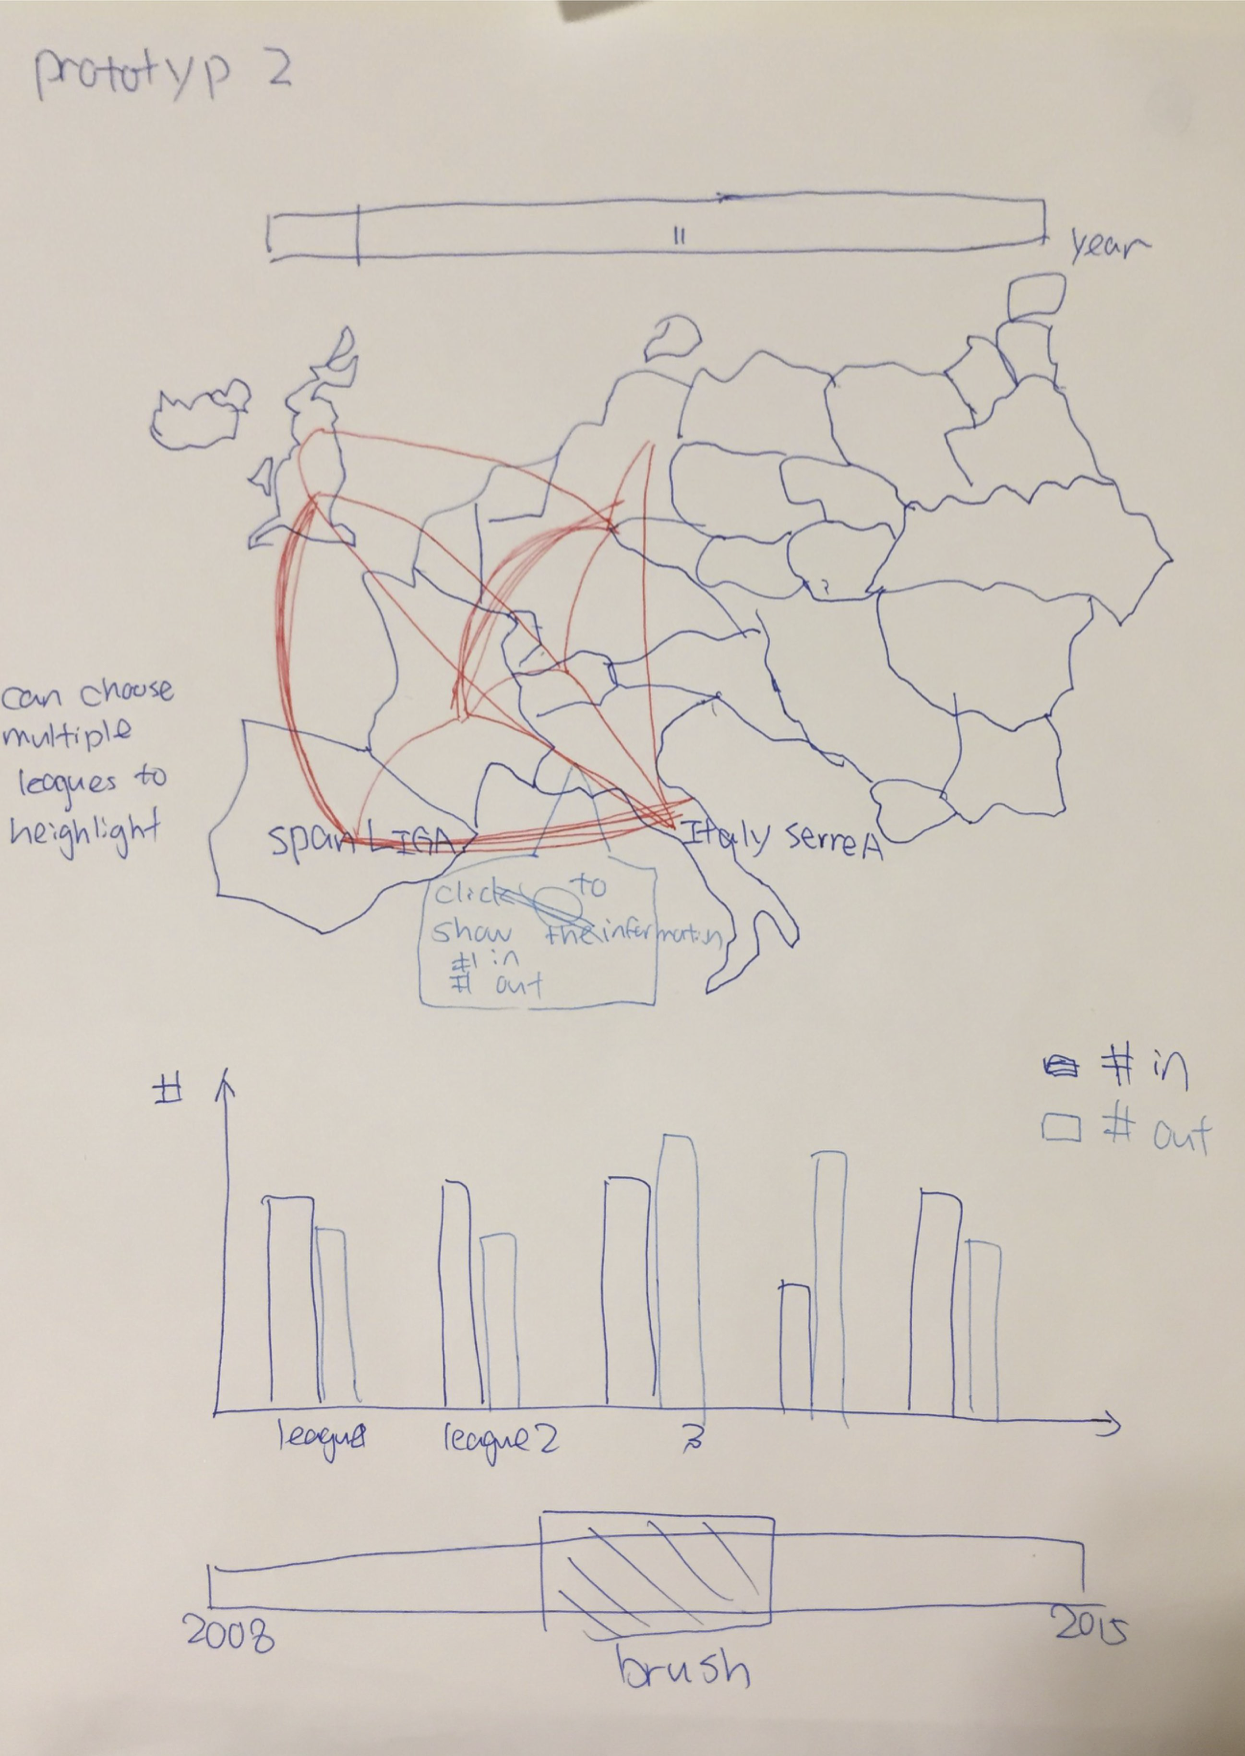
\includegraphics[width=.9\linewidth]{Design5.png}

\begin{itemize}
\item Design3:
\end{itemize}
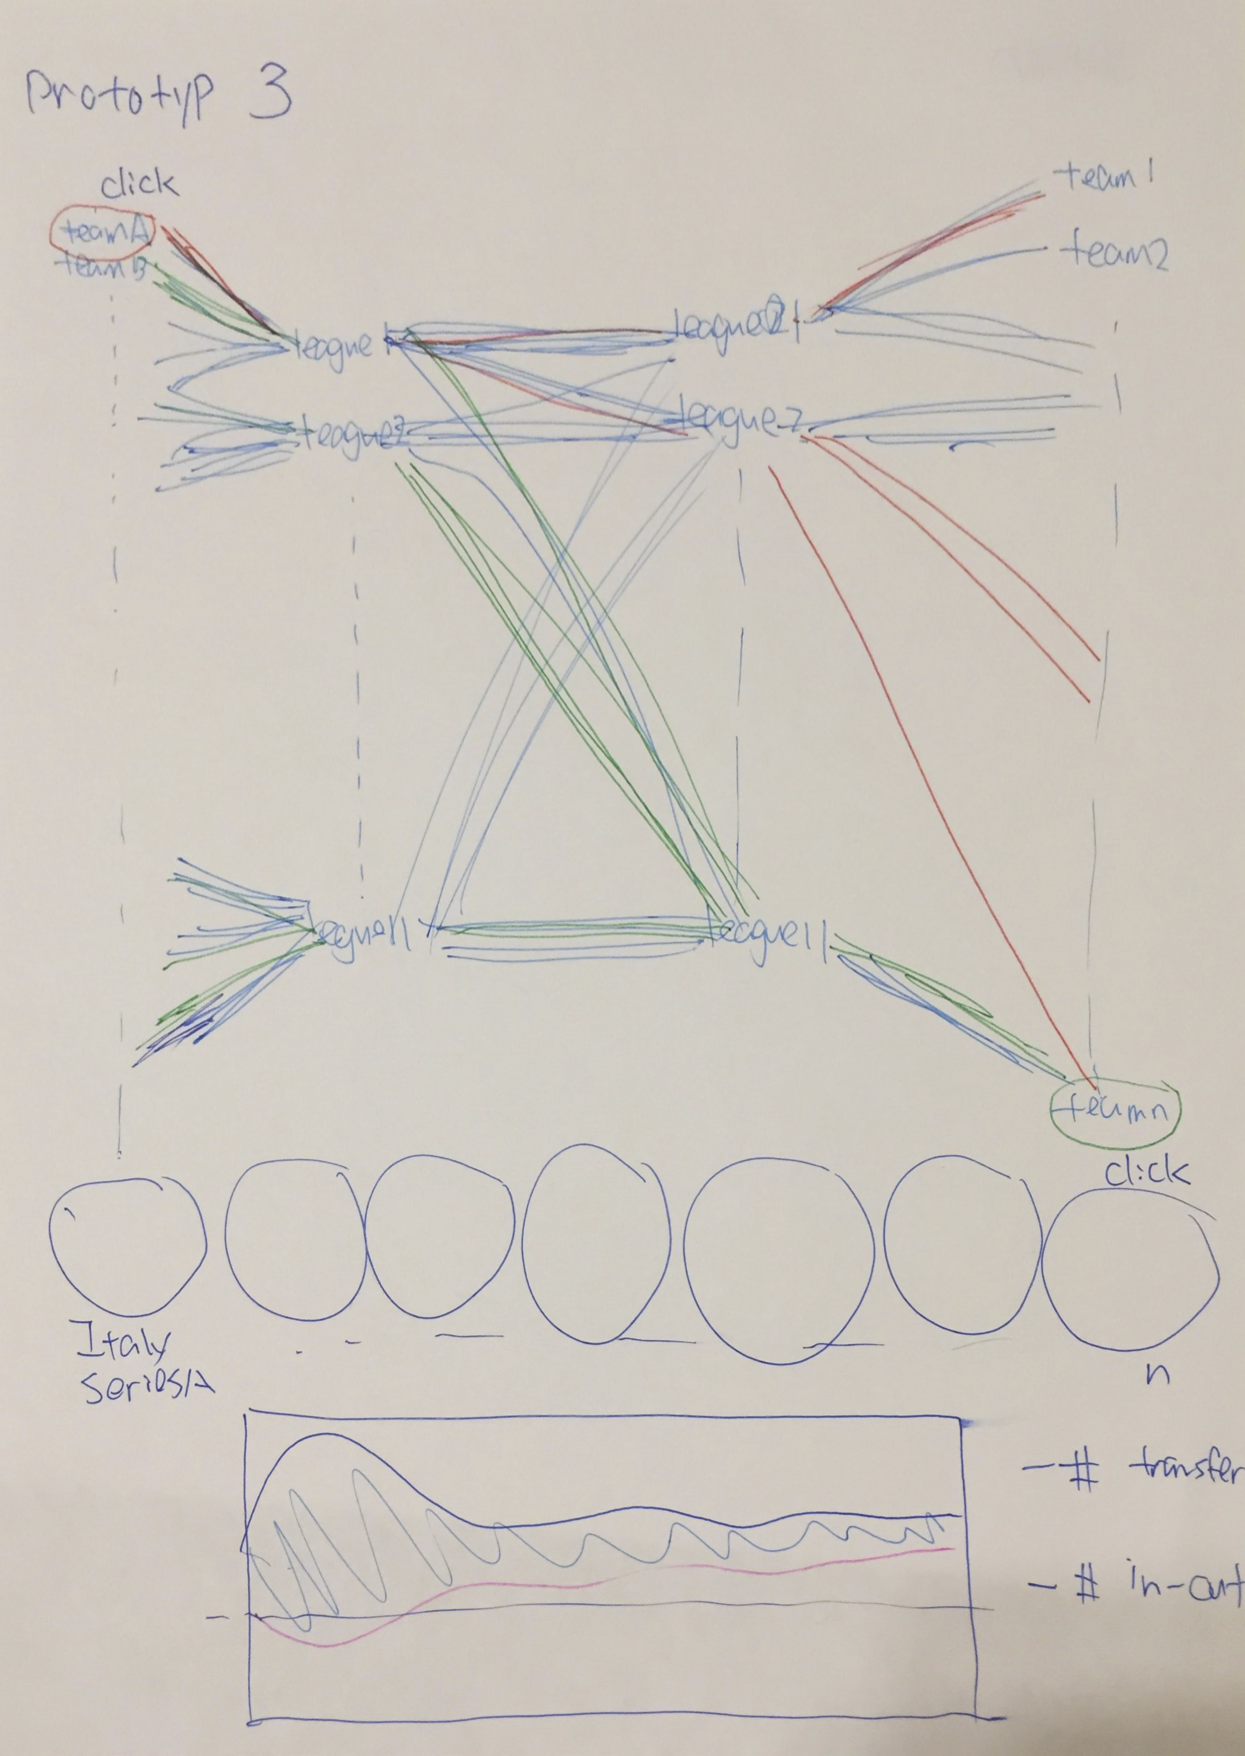
\includegraphics[width=.9\linewidth]{Design6.png}

\subsection{Final Design}
\label{sec-4-3}

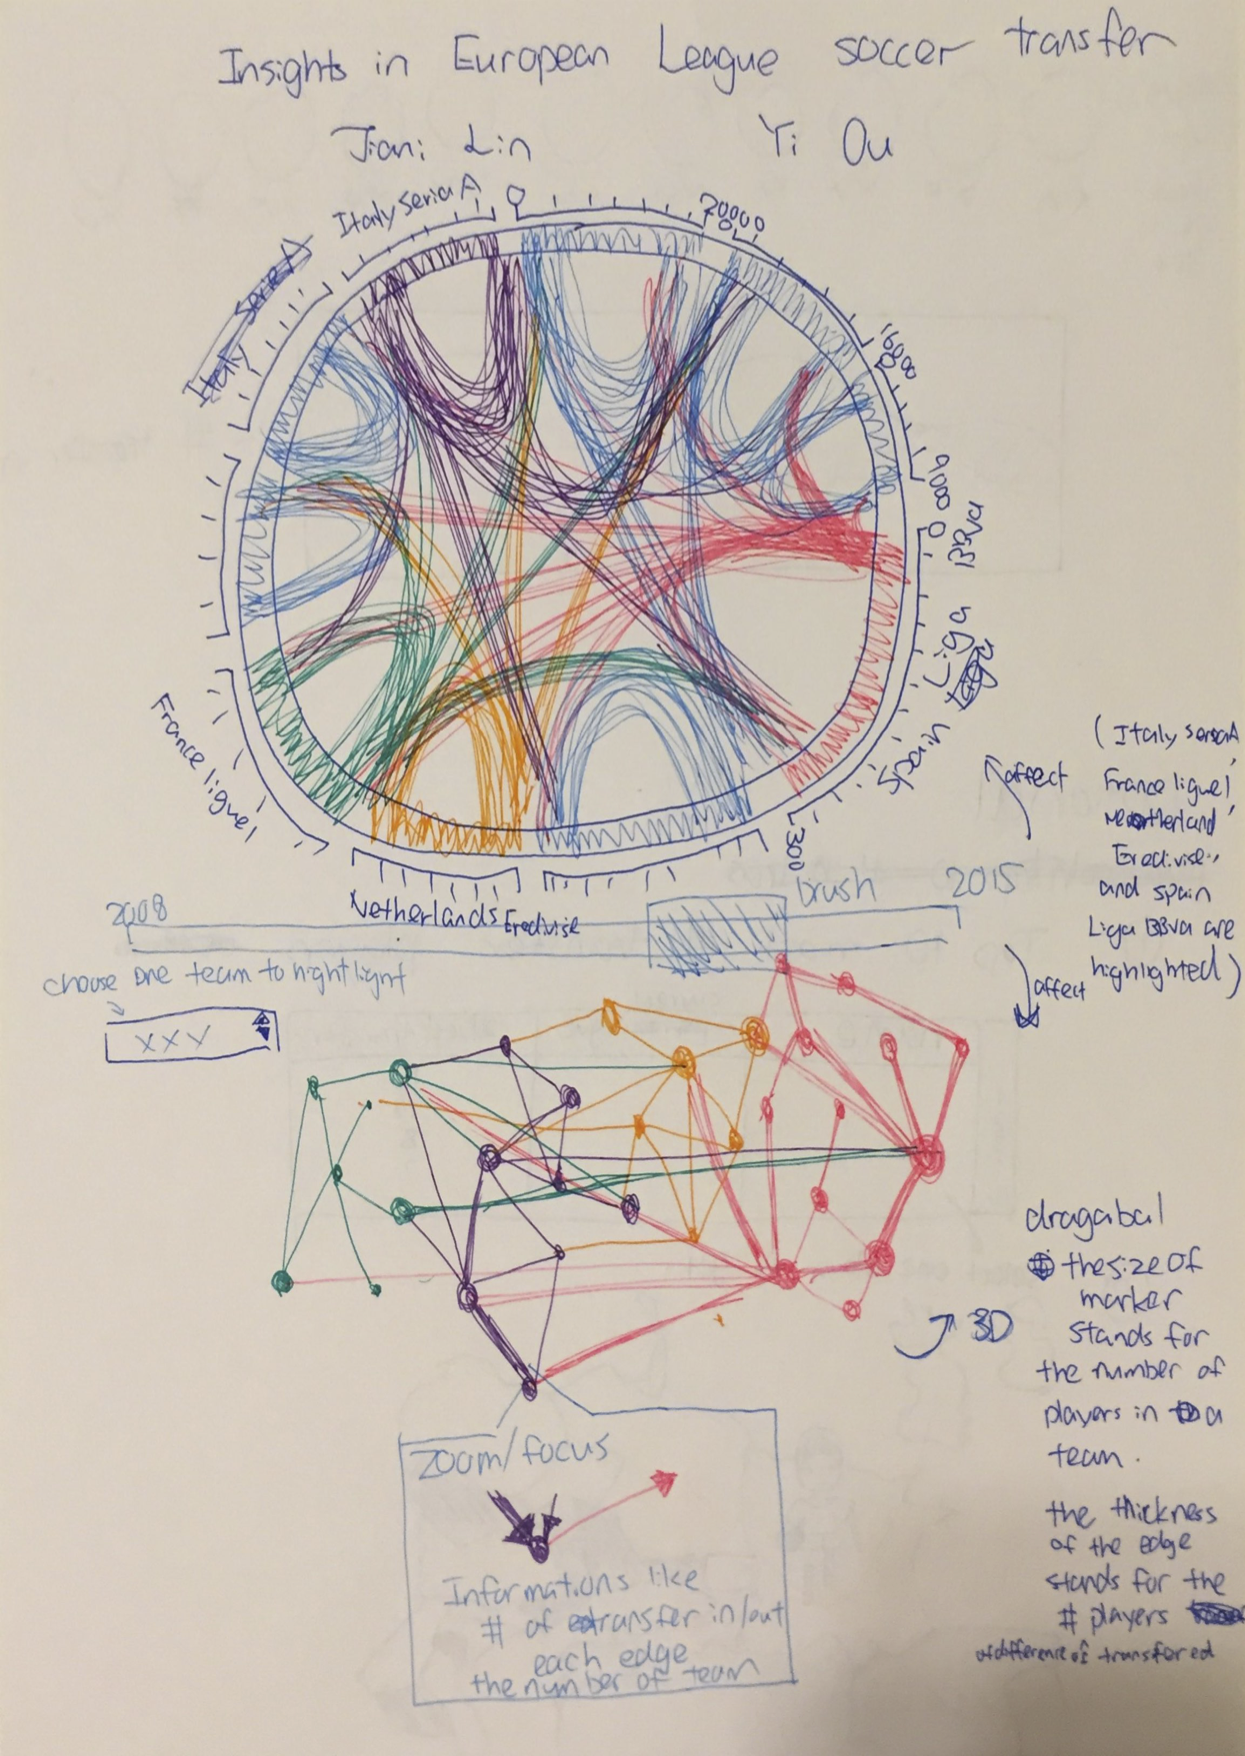
\includegraphics[width=.9\linewidth]{final1.png}

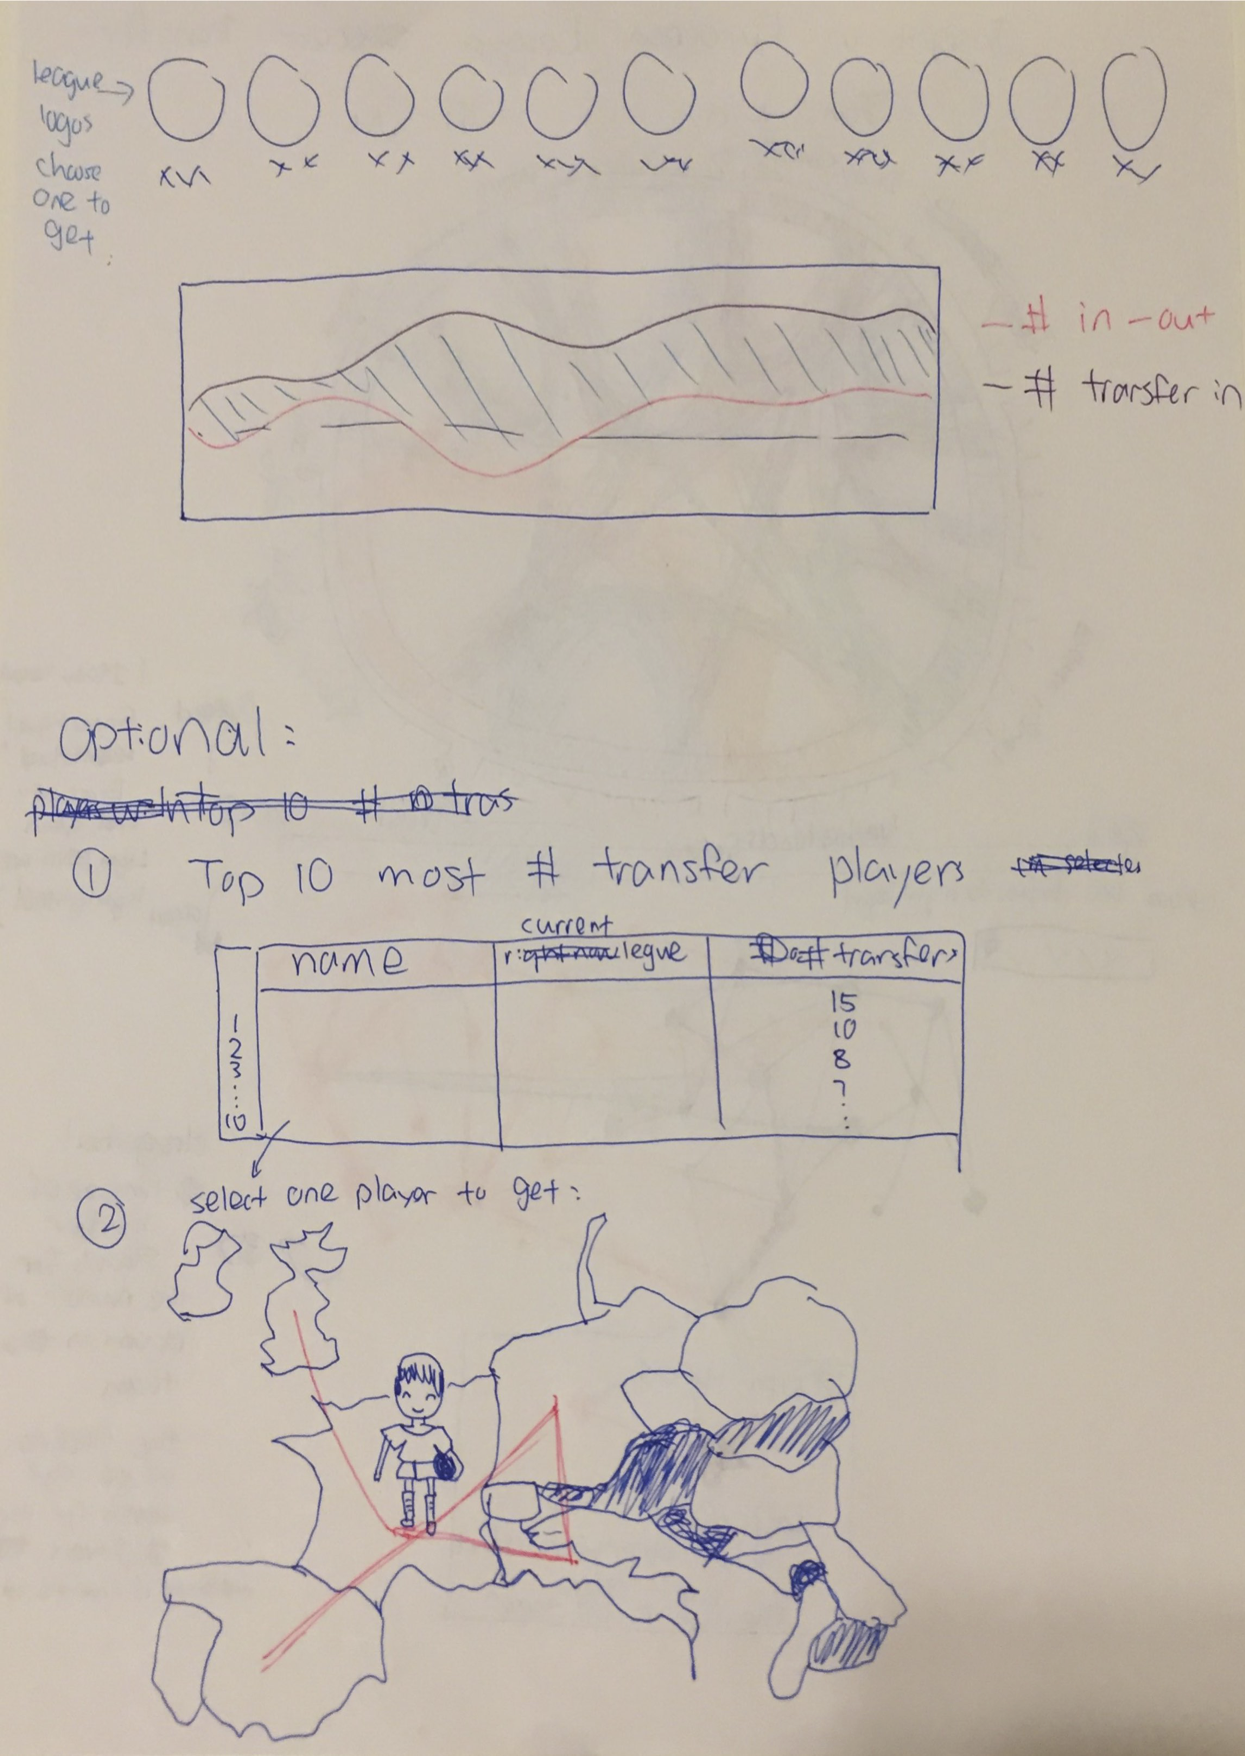
\includegraphics[width=.9\linewidth]{final2.png}

\section{Features}
\label{sec-5}
\subsection{Must-Have}
\label{sec-5-1}
\begin{enumerate}
\item Visualize the number of players transferd between teams within a league in each year.
\item Visualize the number of players transferd between leagues in each year.
\item The trend of players transfer for each league.
\end{enumerate}
\subsection{Optinal}
\label{sec-5-2}
\begin{enumerate}
\item The rank of players who has the most number of transfer times.
\item Animation of players transfer among leagues from year to year.
\item An transfer trace for a selected player.
\end{enumerate}
\section{Schedual}
\label{sec-6}

\begin{center}
\begin{tabular}{lll}
Date & Things to be done & Member\\
\hline
Oct 30 & Data Processing & Yi Ou\\
 & Basic layout & Jiani Lin\\
\hline
Nov 5 & Critical part of feature 1 & Yi OU\\
 & Critical part of feature 2 & Jiani Lin\\
\hline
Nov 11 & Other parts in feature 1 & Yi Ou\\
 & Other parts in feature 2 & Jiani Lin\\
\hline
Nov 17 & Fix or change things based on feedback & Yi Ou\\
 & Critical part of feature 3 & Jiani Lin\\
\hline
Nov 23 & (if everything goes well) Optional feature 1 & Yi Ou\\
 & (if everything goes well) Optional feature 2 & Jiani Lin\\
\hline
Dec 02 & (if everything goes well) Optional feature 3 & Yi Ou\\
 & Final check & Jiani Lin\\
\hline
\end{tabular}
\end{center}
% Emacs 25.1.1 (Org mode 8.2.10)
\end{document}
